\section{Numerical experiments}

To solve the optimal control problem, we use a direct method. %
%
This method considered a time discretization. In this way, if we have a partition $\{\tau_0,\tau_1,\dots,\tau_{N_t}\}$ of interval $[0,\pi/2]$ , we can represent a function $\{ f(\tau) \ | \ \tau \in [0,\pi/2]\}$ as a vector $\bm{f} \in \mathbb{R}^{N_t}$ where component $f_i = f(t_i)$. Then the optimal control problem (\ref{SHEp}) can be written as optimization problem with variable $\bm{f} \in \mathbb{R}^{N_t}$.

\begin{problem}
    Given  $\bm{b}_T  \in \mathbb{R}^{n_b}$,  the optimization problem can be write: 
    \begin{gather}
        \min_{\bm{f} \in \mathbb{R}^{N_t} } \Bigg[ || \bm{b}_T - \bm{\beta}^{N_t}||^2 - \epsilon \Delta\tau  \sum_{i=0}^{N_t} f_{\tau_i}^2 \Bigg]  \\
        \text{suject to: }
        \begin{cases}
            \beta_n^{i+1} = \beta_n^{i} + \Delta \tau (4/\pi) \sin(n\tau_i) f_\tau & \tau \in [0,\pi/2]\label{dyn}\\
            \beta_n^0 = 0
        \end{cases} \\
        \notag \forall n \in \{1,3,5,\dots,N/2 \}
    \end{gather}
\end{problem}

Where we use a euler scheme to discretizate the dynamics. This problem is a Nonlinear programming, for this we use CasADi software to solve.

\subsection{Numerical result for SHE of two levels}

We considered the harmonics $[\beta_1,\beta_5,\beta_7,\beta_{11}]$. We want waveform that  $\bm{b}_T = [b_T^1,b_T^5,b_T^7,b_T^{11}] = [m_a,0,0,0,0]$, where $m_a$ is a parameter . We will compare the different solutions of problem (\ref{SHEp_clas}).
Compararemos el problema mediante soluciones obtenidas del problema (\ref{SHEp_clas}), mediante algoritmos genéticos.

El problema de control óptimo (\ref{OCP1}) reproduce una de las soluciones obtenidas 

\begin{figure}
        \centering
        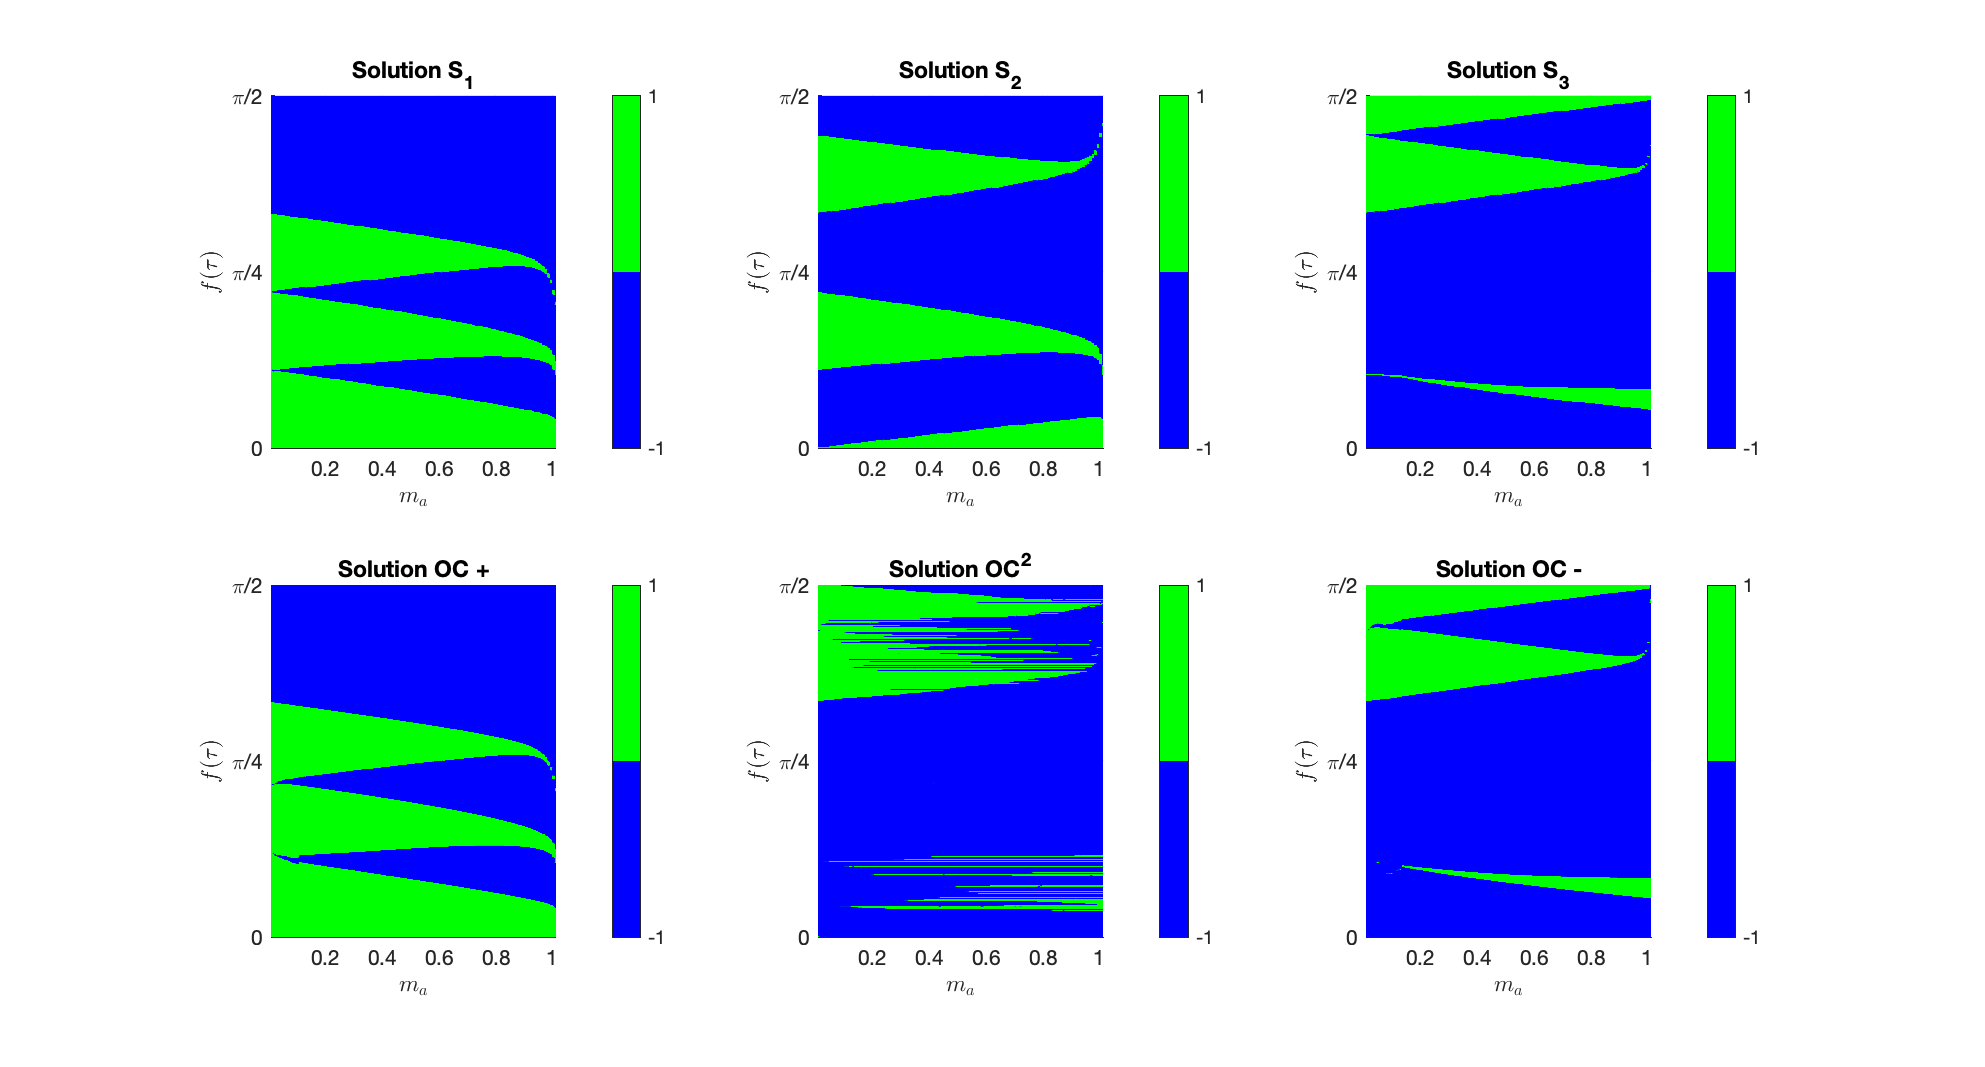
\includegraphics[scale=0.35]{img/EX01_surf.eps}
        \caption{Comparison of solutions for different values of $m_a$. Solutions $S_1$, $S_2$, $S_3$ correspond to problem (\ref{SHEp_clas}) where the number of switching angles is prefixed, while $OC$ solution correspond to optimal control problem.}
        \label{fig:solutions}
    \end{figure}



\begin{figure}
    \centering
    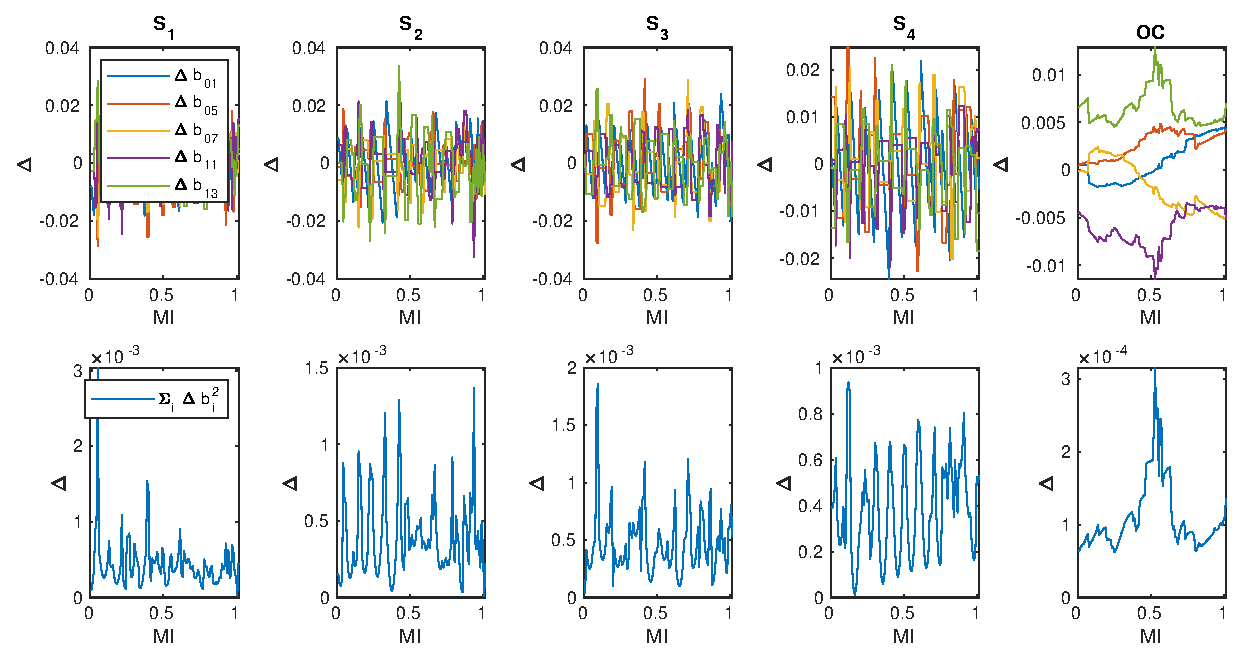
\includegraphics[scale=0.7]{img/EX01.eps}
    \caption{The order of magnitud of the square of euclidean distantes to target is the same for all solutions of figure (\ref{fig:solutions})}
\end{figure}

\subsection{Numerical result for SHE of three levels}

%%%%%%%%%%%%%%%%%%%%%%%%%%%%%%%%%%%%%%%%%%%%%%%%%%%%%%%%%%%

\begin{figure}
    \centering
    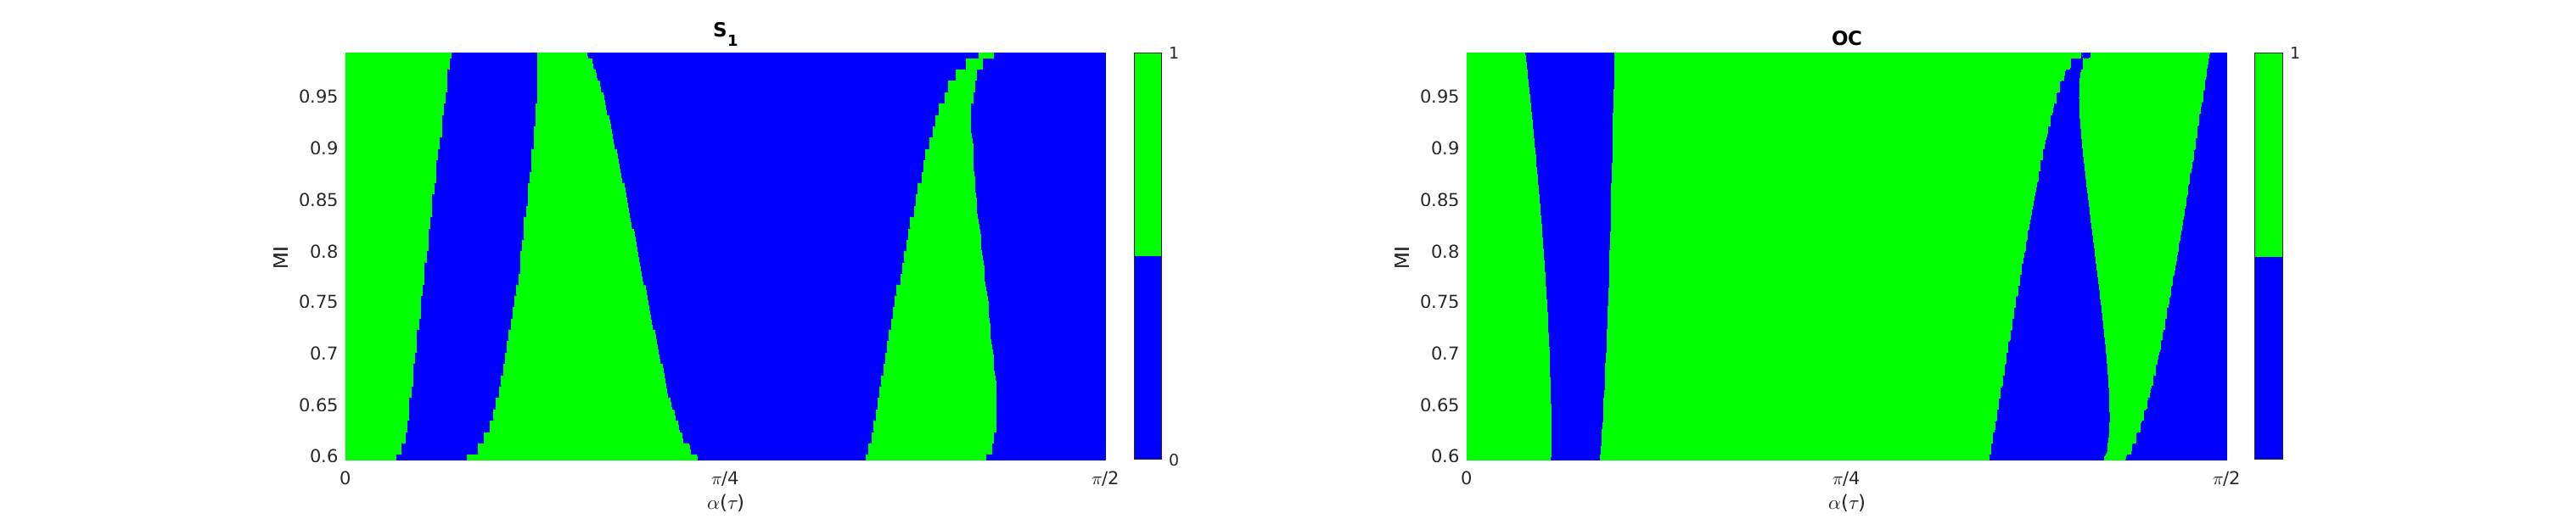
\includegraphics[scale=0.35]{img/EX01_surf_3LVL.eps}
    \caption{Solutions}
\end{figure}



\begin{figure}
    \centering
    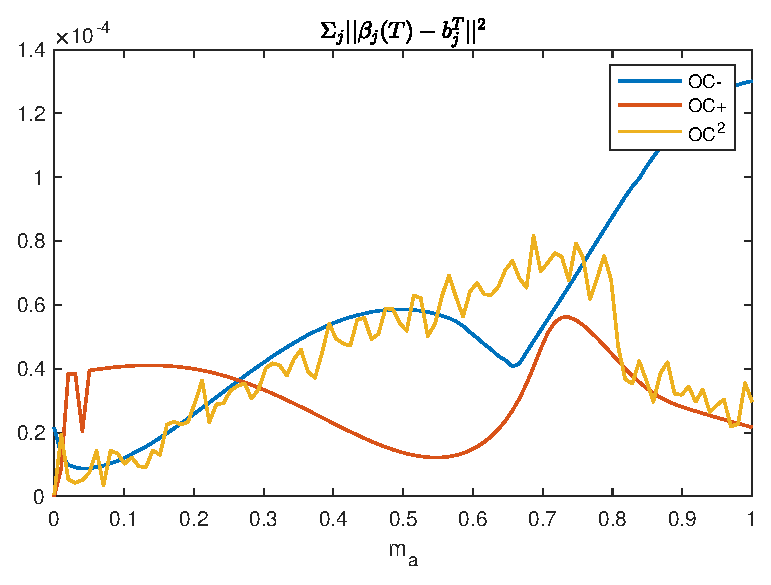
\includegraphics[scale=0.6]{img/EX01_3LVL.eps}
    \caption{Errors}
\end{figure}

